\section{Multi-Fidelity Data}

Multiple analysis techniques with varying fidelity levels are used during the aircraft design process to predict performance characteristics. Earlier in the design process, where there is more freedom in design, lower fidelity analyses allow for quick exploration of the design space. As the design progresses, higher fidelity analyses are used to get a more accurate representation of the aircraft's performance. This general trend is represented in Figure \ref{fig:design_fidelity}.

\begin{figure}
    \center
    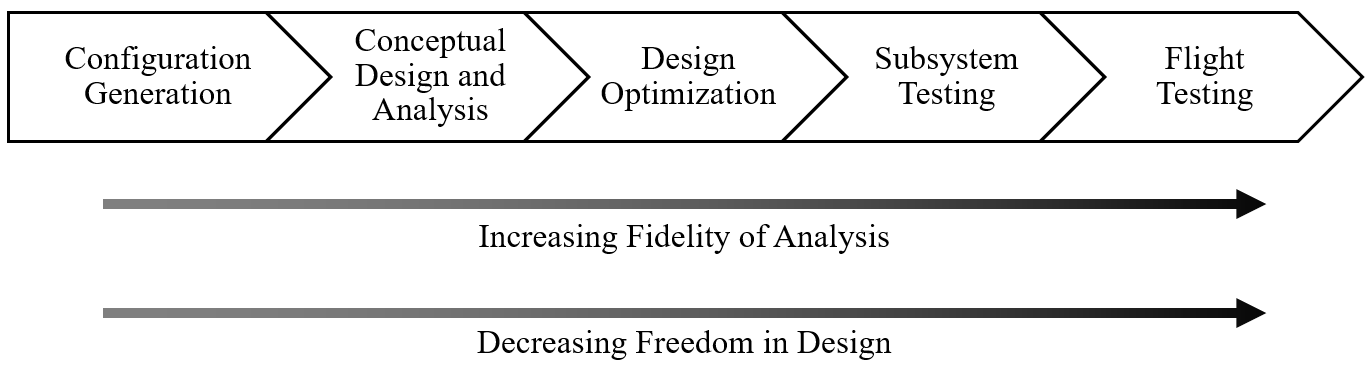
\includegraphics[width=0.95\textwidth]{images/design_fidelity.png}
    \caption{Trends in the aircraft design process and associated design analyses \label{fig:design_fidelity}}
\end{figure}

For this work three analysis increasing fidelity are used: 

\begin{enumerate}
    \item Vortex Lattice analysis (AVL)
    \item RANS CFD (SU2)
    \item Wind tunnel data (NAART, FVWT)
\end{enumerate}

